% prelab4
\documentclass{IEEEtran}
\usepackage{booktabs}
\usepackage{graphicx}
\usepackage{fancyhdr}
\usepackage{framed}
\usepackage{siunitx}
\usepackage{amsmath}
\pagestyle{fancy}
\lhead{}
\chead{}
\rhead{}
\lfoot{}
\cfoot{}
\rfoot{\thepage}
\title{Prelab 4 Second-Order Filters}
\author{Group 8: Muhan Li \and Man Sun \and Mingxiao An \\ EE233 Circuit Theory}
\IEEEaftertitletext{\centering \vspace{-10pt} \fontsize{11}{11}\textsc{Department of Electrical Engineering, University of Washington, Seattle, WA, 98195} \vspace{10pt}}
\begin{document}
	\maketitle
	\section{\textbf{Prelab\#1}}
	We can redraw the circuit as figure[\ref{fig:1.1}]. Then we have the following equations according to KCL.\\
	\begin{figure}[!htbp]
		\centering
		\begin{framed}
			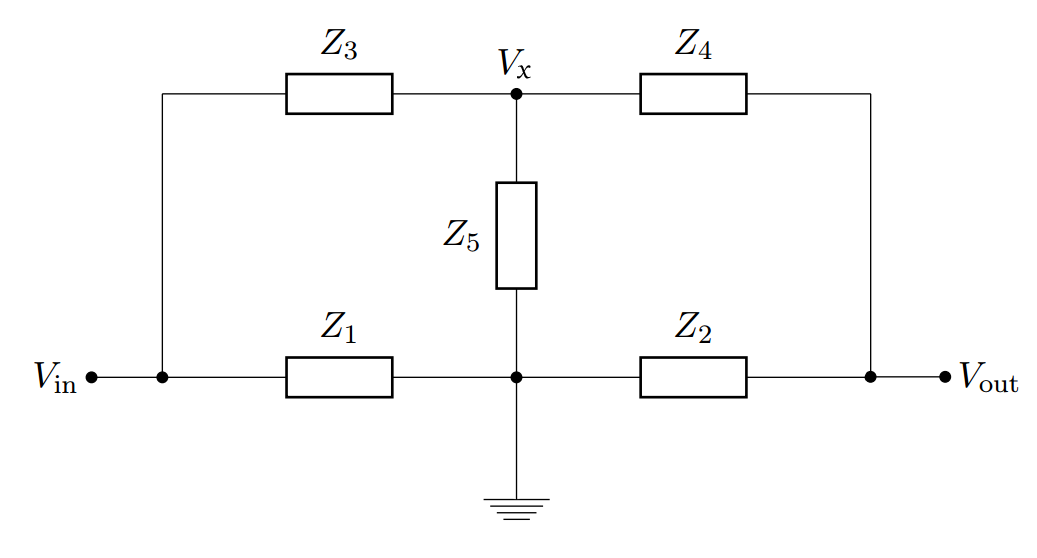
\includegraphics[width=\linewidth]{images/1_1.png}
			\caption{An equivalent circuit for prelab \#1}
			\label{fig:1.1}
		\end{framed}
	\end{figure}
	\begin{eqnarray*}
	\frac{V_x}{Z_5} + \frac{V_{in}}{Z_1}+\frac{V_{out}}{Z_2} & = & 0\\
	\frac{V_{in}-V_x}{Z_3} + \frac{V_{out}-V_x}{Z_4} - \frac{V_x}{5} & = & 0\\
	V_x(\frac{1}{Z_3}+\frac{1}{Z_4}+\frac{1}{Z_5})  + \frac{V_{in}}{Z_3}+\frac{V_{out}}{Z_4} & = & 0\\
	\mathrm{Let}\quad Y_t \quad=\quad \frac{1}{Z_3}+\frac{1}{Z_4}+\frac{1}{Z_5} & & \\
	(\frac{V_{in}}{Z_3}+\frac{V_{out}}{Z_4})\frac{1}{Y_tZ_5} + \frac{V_{in}}{Z_1} +\frac{V_{out}}{Z_2} & = & 0\\
	V_{in}(\frac{1}{Z_3Z_5Y_t}+\frac{1}{Z_1}) + V_{out}(\frac{1}{Z_4Z_5Y_t} + \frac{1}{Z_2}) & = & 0	
	\end{eqnarray*}
	\begin{eqnarray*}
		H(s) \quad=\quad \frac{V_{out}}{V_{in}} & = & -\frac{\frac{1}{Z_3Z_5Y_t}+\frac{1}{Z_1}}{\frac{1}{Z_4Z_5Y_t}+\frac{1}{Z_2}}\\
		& = & - \frac{\frac{1}{Z_3}+\frac{Z_5Y_t}{Z_1}}{\frac{1}{Z_4}+\frac{Z_5Y_t}{Z_2}}\\
		& = & - \frac{\frac{1}{Z_3}+\frac{Z_5}{Z_1}(\frac{1}{Z_3}+\frac{1}{Z_4}+\frac{1}{Z_5})} {\frac{1}{Z_4}+\frac{Z_5}{Z_2}(\frac{1}{Z_3}+\frac{1}{Z_4}+\frac{1}{Z_5})}
	\end{eqnarray*}
	\section{\textbf{Prelab\#2}}
	In terms of Z\\
	\begin{eqnarray*}
		H(s) & = & -\frac{\frac{Z}{Z_3}+Z_5(\frac{1}{Z_3}+\frac{1}{Z_4}+\frac{1}{Z_5})} {\frac{Z}{Z_4}+Z_5(\frac{1}{Z_3}+\frac{1}{Z_4}+\frac{1}{Z_5})}\\
		& = &-\frac{ZZ_4+Z_3Z_4Z_5(\frac{1}{Z_3}+\frac{1}{Z_4}+\frac{1}{Z_5})} {ZZ_3+Z_3Z_4Z_5(\frac{1}{Z_3}+\frac{1}{Z_4}+\frac{1}{Z_5})}\\	
	\end{eqnarray*}
	\phantom{ } We can let $ Z_3 = Z_4 $, so that $ |H(s)| = 1 $.
	\section{\textbf{Prelab\#3}}
	\subsection{the frequency response}
	\begin{eqnarray*}
		H(s) & = & -\frac{Z + Z_3Z_5(\frac{1}{Z_3}+\frac{1}{Z_4}+\frac{1}{Z_5})} {Z\frac{Z_3}{Z_4}+Z_3Z_5(\frac{1}{Z_3}+\frac{1}{Z_4}+\frac{1}{Z_5})}\\
		& = & - \frac{2400+100000-\frac{3\times10^8}{\omega}\mathbf{j}} {4800+100000-\frac{3\times10^8}{\omega}\mathbf{j}}\\
		& = & - \frac{102.4\omega - 300\mathrm{k}\mathbf{j}}{104.8\omega - 300\mathrm{k}\mathbf{j}}\\
	\end{eqnarray*}
	\subsection{the gain of the filter}
	See figure[\ref{fig:3.1}].
	
	\begin{figure}[!htbp]
		\centering
		\begin{framed}
			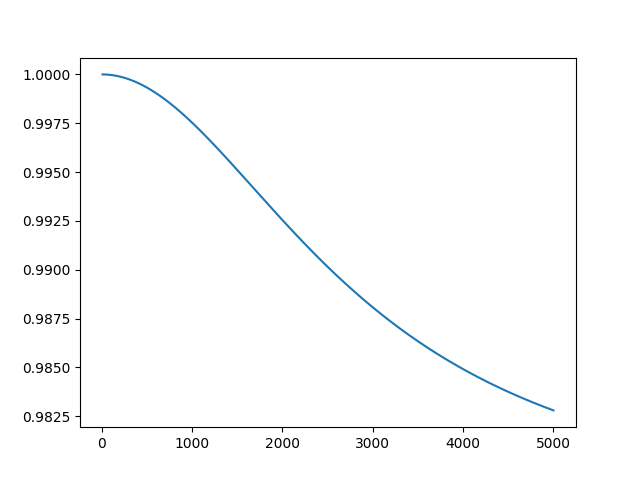
\includegraphics[width=\linewidth]{images/3_1.png}
			\caption{Gain of the filter in prelab \#3}
			\label{fig:3.1}
		\end{framed}
	\end{figure}

	\subsection{the gain of the filter after switching $ R_3 $ and $ R_4 $}
	After switching $ R_3 $ and $ R_4 $, we have\\
	\begin{eqnarray*}
		H(s) & = & -\frac{Z + Z_4Z_5(\frac{1}{Z_3}+\frac{1}{Z_4}+\frac{1}{Z_5})} {Z\frac{Z_4}{Z_5}+Z_4Z_5(\frac{1}{Z_3}+\frac{1}{Z_4}+\frac{1}{Z_5})}\\
		& = & - \frac{4800+100000-\frac{3\times10^8}{\omega}\mathbf{j}} {2400+100000-\frac{3\times10^8}{\omega}\mathbf{j}}\\
		& = & - \frac{104.8\omega - 300\mathrm{k}\mathbf{j}}{102.4\omega - 300\mathrm{k}\mathbf{j}}\\
	\end{eqnarray*}
	See figure[\ref{fig:3.2}].
	
	\begin{figure}[!htbp]
		\centering
		\begin{framed}
			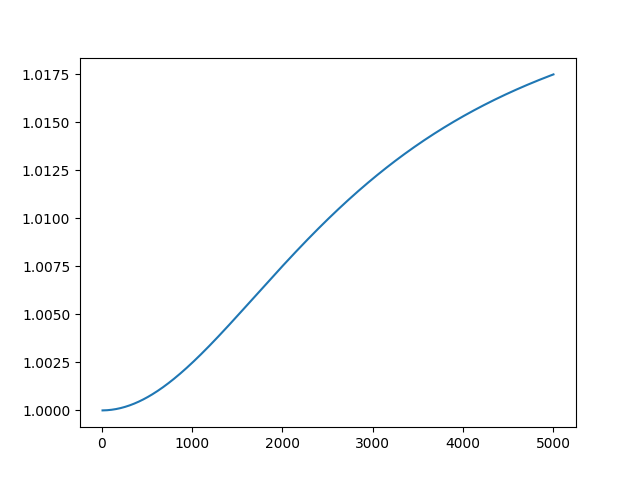
\includegraphics[width=\linewidth]{images/3_2.png}
			\caption{Gain after switching $ R_3 $ and $ R_4 $}
			\label{fig:3.2}
		\end{framed}
	\end{figure}

	\section{\textbf{Prelab\#4}}
	Let $ H(s) $ be the frequency response of the filter, and let $ H^\prime(s) $ be the frequency response of the filter after switching $ R_3 $ and $ R_4 $, we have\\
	\begin{equation*}
		H(s)\cdot H^\prime(s) = 1
	\end{equation*}
	\phantom{ } So we can conclude that the type of the filter after switching $ R_3 $ and $ R_4 $ is just the opposite type of the filter before the two resistors are switched. For example, if the filter is low-pass, it will become high-pass; if the filter is high-pass, it will become low-pass; it the filter is band-pass, it will become band-stop.
	
	\section{\textbf{Prelab\#5}}
	Let $ Z_1 = \gamma R_5 $, where $ 0 \le \gamma \le 1 $, we have $ Z_2 = (1-\gamma)R_5 $ and the following equations:\\
	\begin{eqnarray*}
		Z_3 & = & \frac{1}{sC_1}\\
		Z_a & = & \frac{(1-\gamma)R_5\cdot\frac{1}{sC_1}}{R_5+\frac{1}{sC_1}}\\
			& = & \frac{(1-\gamma) R_5}{sR_5C_1+1}\\
		Z_b & = & \frac{\gamma R_5}{sR_5C_1+1}\\
		Z_c & = & \frac{\gamma (1-\gamma)R_5^2sC_1}{sR_5C_1+1}\\
	\end{eqnarray*}
	Our schematic is shown in figure[].
	
	\section{\textbf{Prelab\#6}}
	\begin{eqnarray*}
		Z_3 & = & R_3 + Z_a\\
		Z_4 & = & R_4 + Z_b\\
		Z_5 & = & \frac{1}{sC_2} + Z_c\\
		H(s) & = & - \frac{\frac{1}{R_3 + Z_a}+\frac{\frac{1}{sC_2} + Z_c}{Z_1} (\frac{1}{R_3 + Z_a}+\frac{1}{R_4 + Z_b}+\frac{1}{\frac{1}{sC_2} + Z_c})} {\frac{1}{R_4 + Z_b}+\frac{\frac{1}{sC_2} + Z_c}{Z_2}(\frac{1}{R_3 + Z_a}+\frac{1}{R_4 + Z_b}+\frac{1}{\frac{1}{sC_2} + Z_c})}
	\end{eqnarray*}
	\section{\textbf{Prelab\#7}}
	\hfil \newline
	\phantom{ } For 250$ \si{\hertz} $, we let $ C_1 = 0.1\mu\si{\farad} $, $ C_2 = 0.0050\mu\si{\farad} $.\\
	\phantom{ } For 1$ \si{\kilo\hertz} $, we let $ C_1 = 0.022\mu\si{\farad} $, $ C_2 = 0.0022\mu\si{\farad} $.\\
	\phantom{ } For 4$ \si{\kilo\hertz} $, we let $ C_1 = 0.0050\mu\si{\farad} $, $ C_2 = 500\si{\pico\farad} $.\\
	\phantom{ } Our matlab result is shown in figure[\ref{fig:7.1},\ref{fig:7.2},\ref{fig:7.3}].
	\begin{figure}[!htbp]
		\centering
		\begin{framed}
			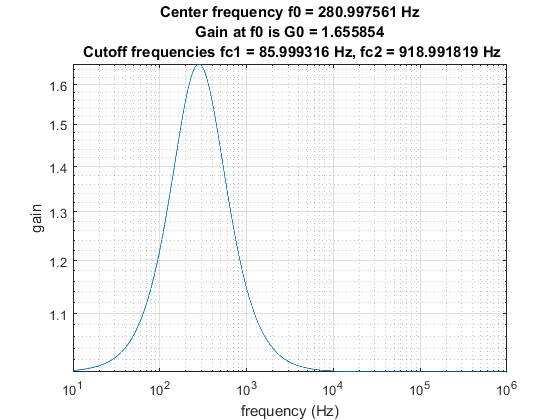
\includegraphics[width=\linewidth]{images/7_1.png}
			\caption{band-pass filter with center frequency around 250Hz}
			\label{fig:7.1}
		\end{framed}
	\end{figure}
	\begin{figure}[!htbp]
		\centering
		\begin{framed}
			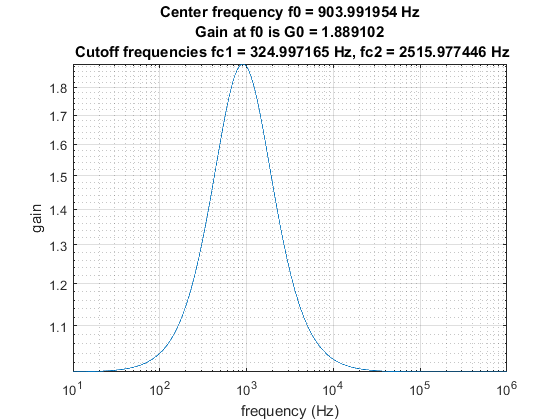
\includegraphics[width=\linewidth]{images/7_2.png}
			\caption{band-pass filter with center frequency around 400Hz}
			\label{fig:7.2}
		\end{framed}
	\end{figure}
	\begin{figure}[!htbp]
		\centering
		\begin{framed}
			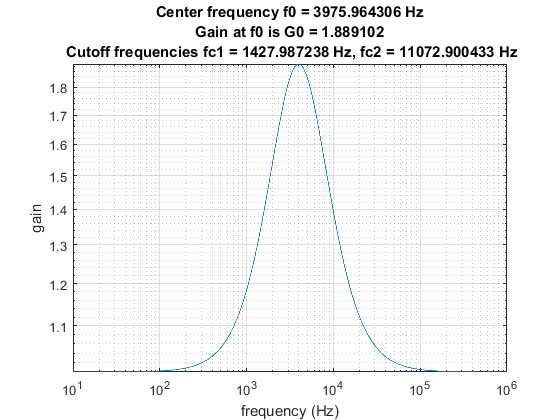
\includegraphics[width=\linewidth]{images/7_3.png}
			\caption{band-pass filter with center frequency around 4kHz}
			\label{fig:7.3}
		\end{framed}
	\end{figure}
	\section{\textbf{Prelab\#8}}
	We set the values for two capacitors separately and got the simulated plots for the three filters. We plotted the gain Bode plot for these three filters separately in figure[\ref{fig:8.1},\ref{fig:8.2},\ref{fig:8.3}]. And we used cursor to record the center frequency, cutoff frequency and gain(peak). These data were shown in table[\ref{tab:ACpara}].
	\begin{figure}[!htbp]
		\centering
		\begin{framed}
			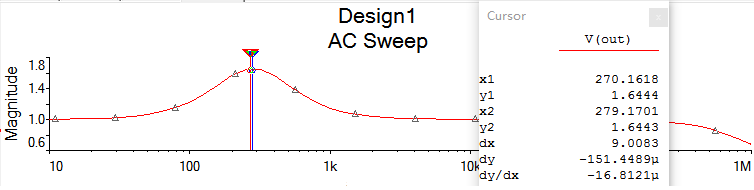
\includegraphics[width=\linewidth]{images/8_1.PNG}
			\caption{SPICE Bode plot for the first filter}
			\label{fig:8.1}
		\end{framed}
	\end{figure}
	\begin{figure}[!htbp]
		\centering
		\begin{framed}
			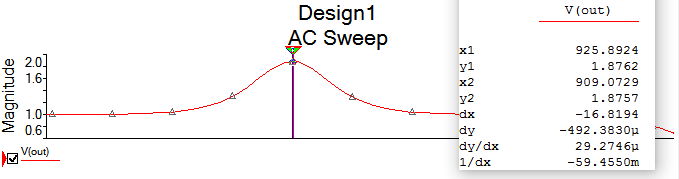
\includegraphics[width=\linewidth]{images/8_2.PNG}
			\caption{SPICE Bode plot for the second filter}
			\label{fig:8.2}
		\end{framed}
	\end{figure}
	\begin{figure}[!htbp]
		\centering
		\begin{framed}
			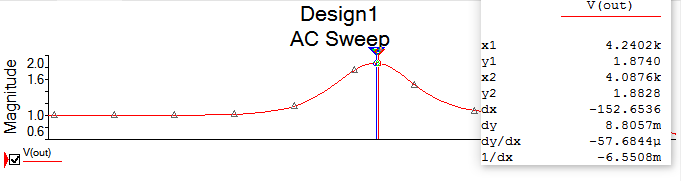
\includegraphics[width=\linewidth]{images/8_3.PNG}
			\caption{SPICE Bode plot for the third filter}
			\label{fig:8.3}
		\end{framed}
	\end{figure}

	\begin{table}[!htbp]
		\centering
		\caption{Some AC parameters for the three filters}
		\begin{tabular}{lcccc}
			\toprule
			No &center freq($\si{\hertz}$) &cutoff freq1($\si{\hertz}$)&cutoff freq2($ \si{\hertz} $)&peak gain\\
			\midrule
			1	&281.22	&82.339	&943.02	&1.6443\\
			2	&996.34	&319.73	&2538.7	&1.8781\\
			3	&4013.3	&1411.5	&11000	&1.8872\\
			\bottomrule
		\end{tabular}
		\label{tab:ACpara}
	\end{table}	
\end{document}